\subsection{Induced electric current}
	%Redo this part if necessary
	The plasma is flowing in in relation to the coordinate system in the simulations.
	Due to this an induced electrical field, \(\varepsilon\), will appear.
	The induced electrical field will neutralize the Lorentz force.
	Combined with the electrostatic approximation we can obtain the \(\varepsilon\)

	\begin{equation}
		\vec{\varepsilon} = \vec{v_D}\times \vec{B}
	\end{equation}

	\begin{equation}
		\int{Edx} = -\phi
	\end{equation}

	\begin{equation}
		\phi = -\int \vec{v}_d\times\vec{B} \approx -\int \left( 41600 \text{m/s}\cdot 50E-6 \text{T} \right) dx
	\end{equation}
	\begin{equation}
		\phi = -2.08 \text{x} + C
	\end{equation}

\subsection{Paths of the photoemmited electrons}
	The electrons emmited from the spacecraft due to the photoelectric effect, have a kinetic
	energy corresponding to a Maxwellian distribution with a temperature of \(T_{ph} =  3.8481\cdot 10^{4} \text{K}\).
	Figure~\ref{fig:trajectories} illustrates the trajectories of the emmited electrons in simulation \(6\).
	As the probes are situated \(10 \text{cm}\) to the sides of the spacecraft on the \(x-\)axis, the probes
	may be hit by the photo-emmited electrons. In the following section, \ref{sec:acc_emmited}, we show the number of electrons hitting
	the probes.


	\begin{figure}
		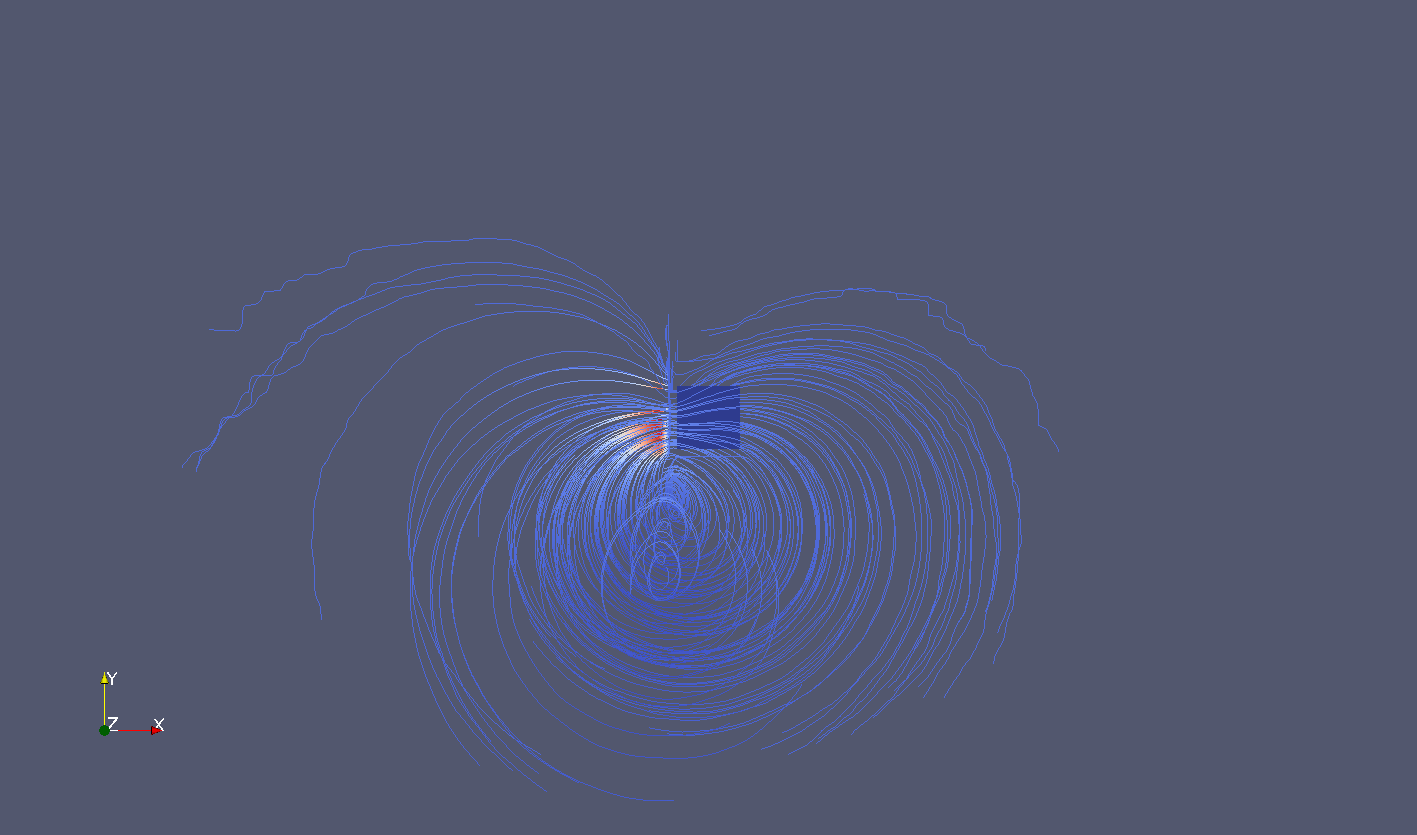
\includegraphics[width = 0.49 \textwidth]{images/case6_jph_paths}
		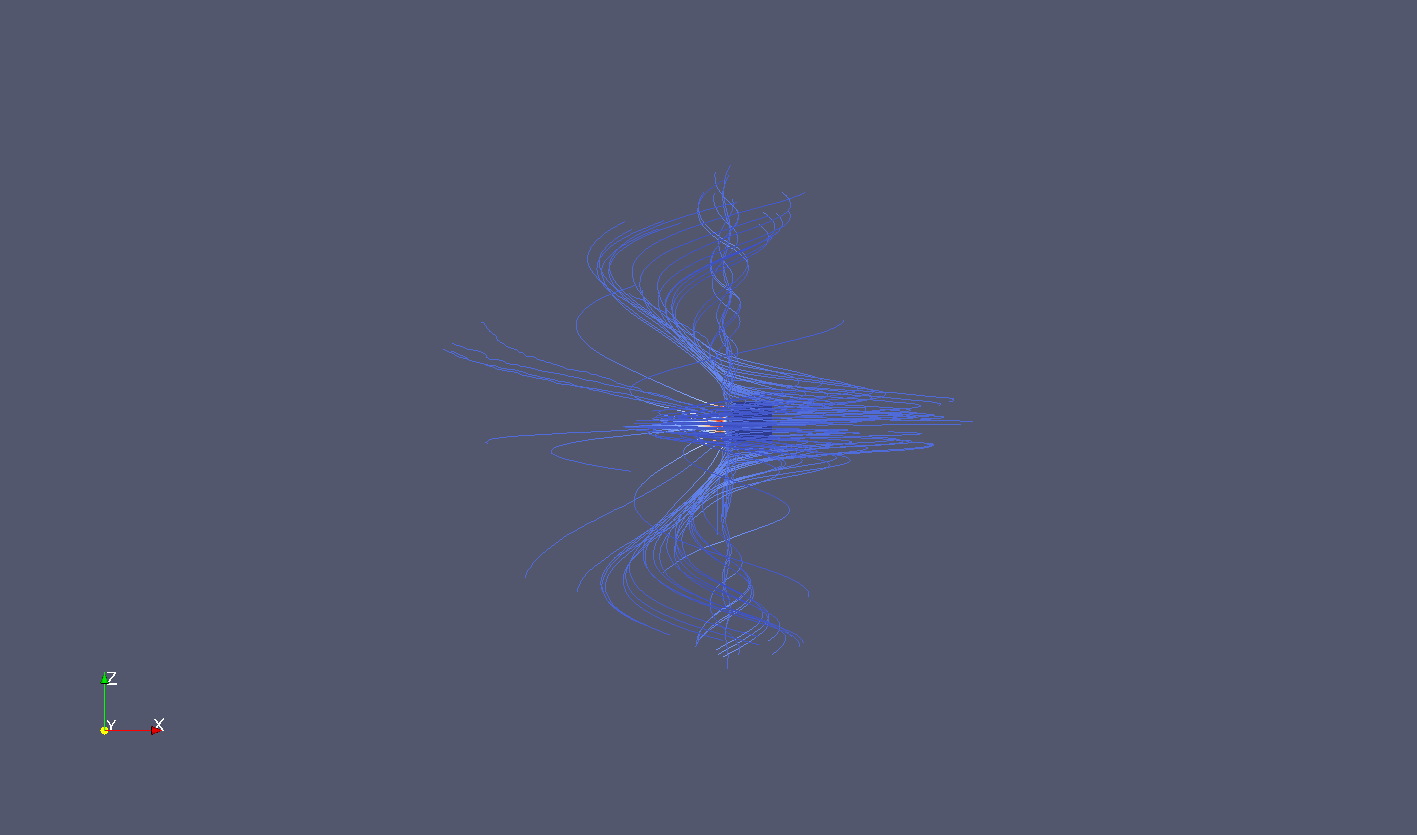
\includegraphics[width = 0.49 \textwidth]{images/case6_jph_paths_2}
		\caption{The trajectories of the electrons emmited by the photoelectric effect in simulation \(6\). The possible
 		paths of the photoemmited electrons coincide with the volume occupied by the langmuir probes. The photoemmited electrons are strongly affected by the magnetic
		field \(\vec{B}\), and follows a gyrating path guided by \(\vec{B}\). The photoemmited electrons are in all the studied cases
		emmited from the spacecraft in \(-x\) direction, and the paths are similar. The langmuir probes are situated \(10 \text{cm}\) to each side
		of the spacecraft along the \(x-\)direction. (NOTE, should have axis labels, and domain length.)}
		\label{fig:trajectories}
 	\end{figure}


\subsection{Potential difference with P-E and no P-E}

    \begin{figure}
        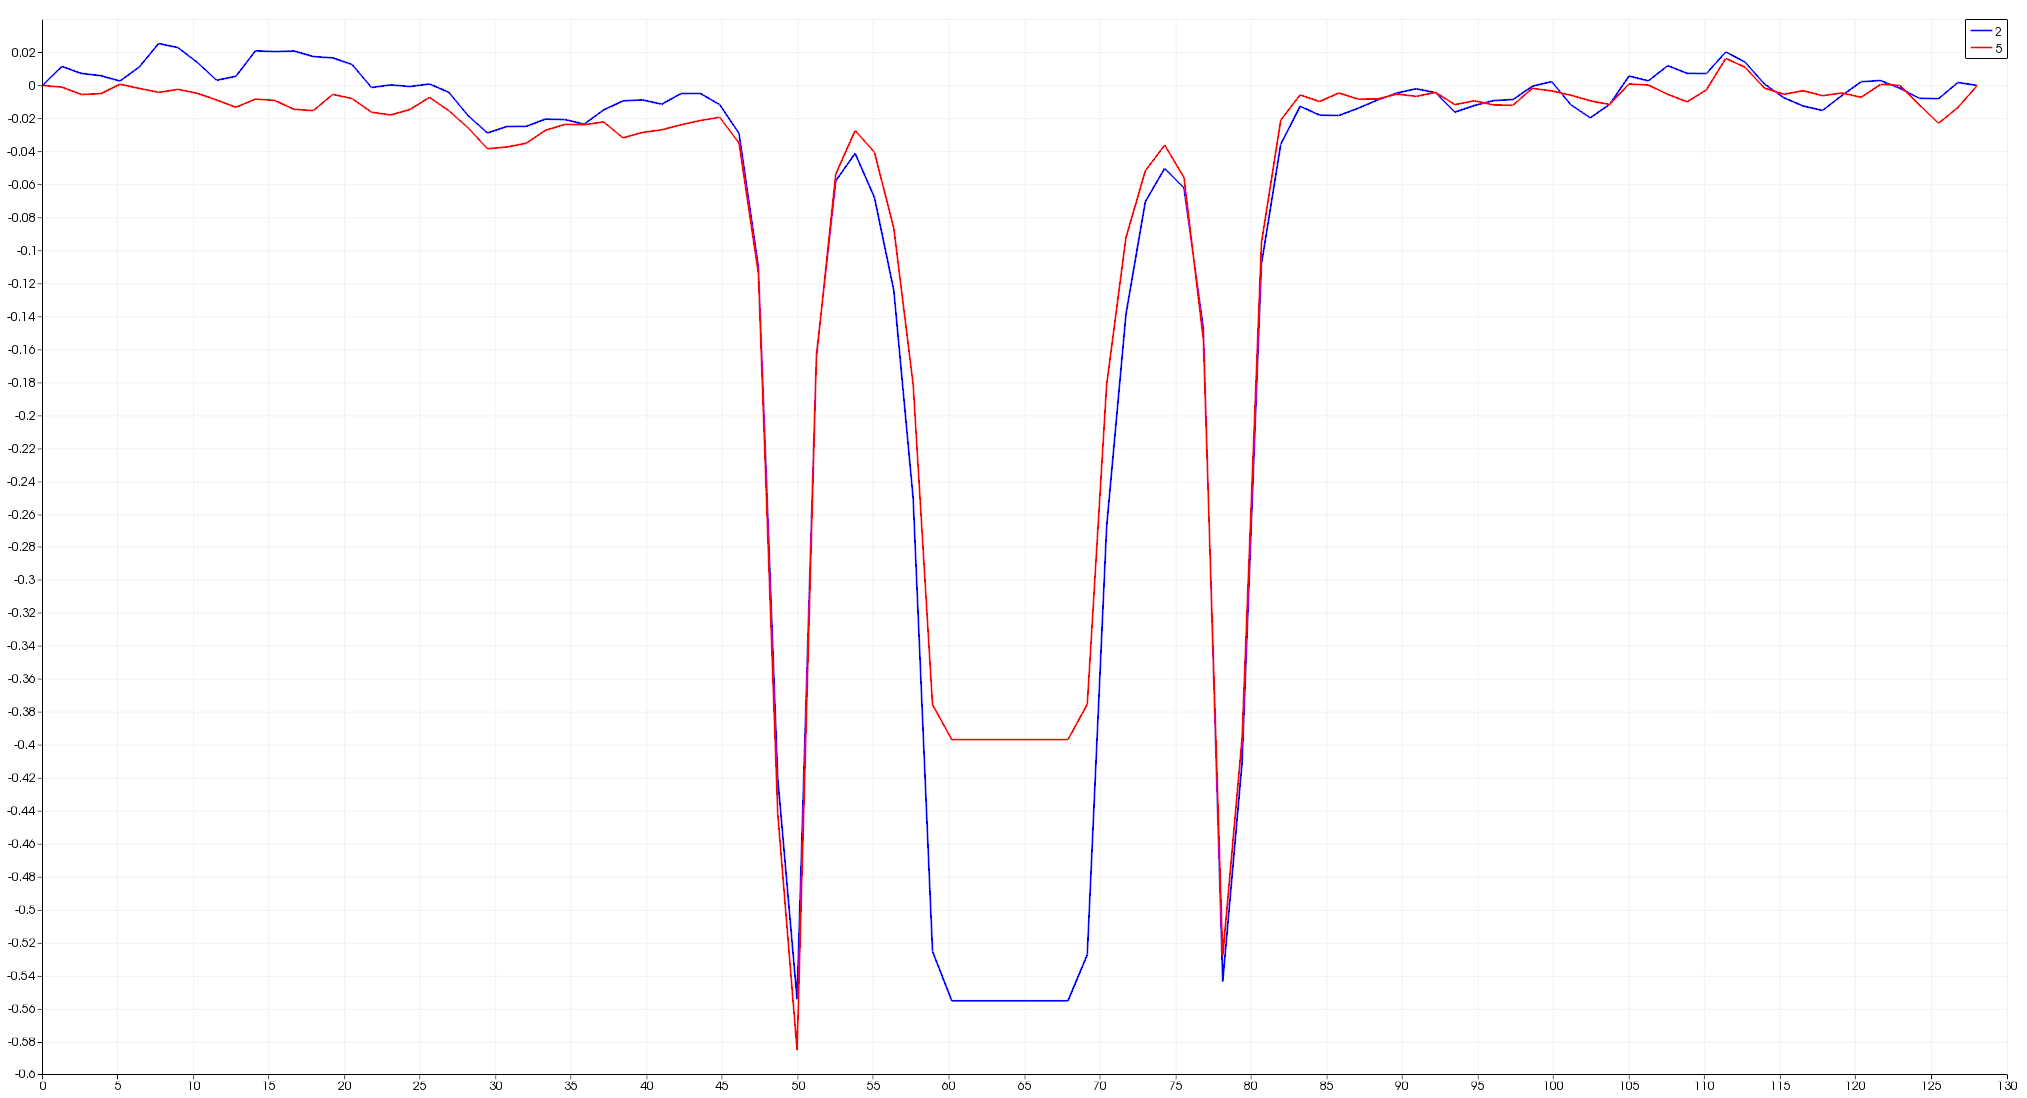
\includegraphics[width = 0.3 \textwidth]{images/pot_case25.png}
        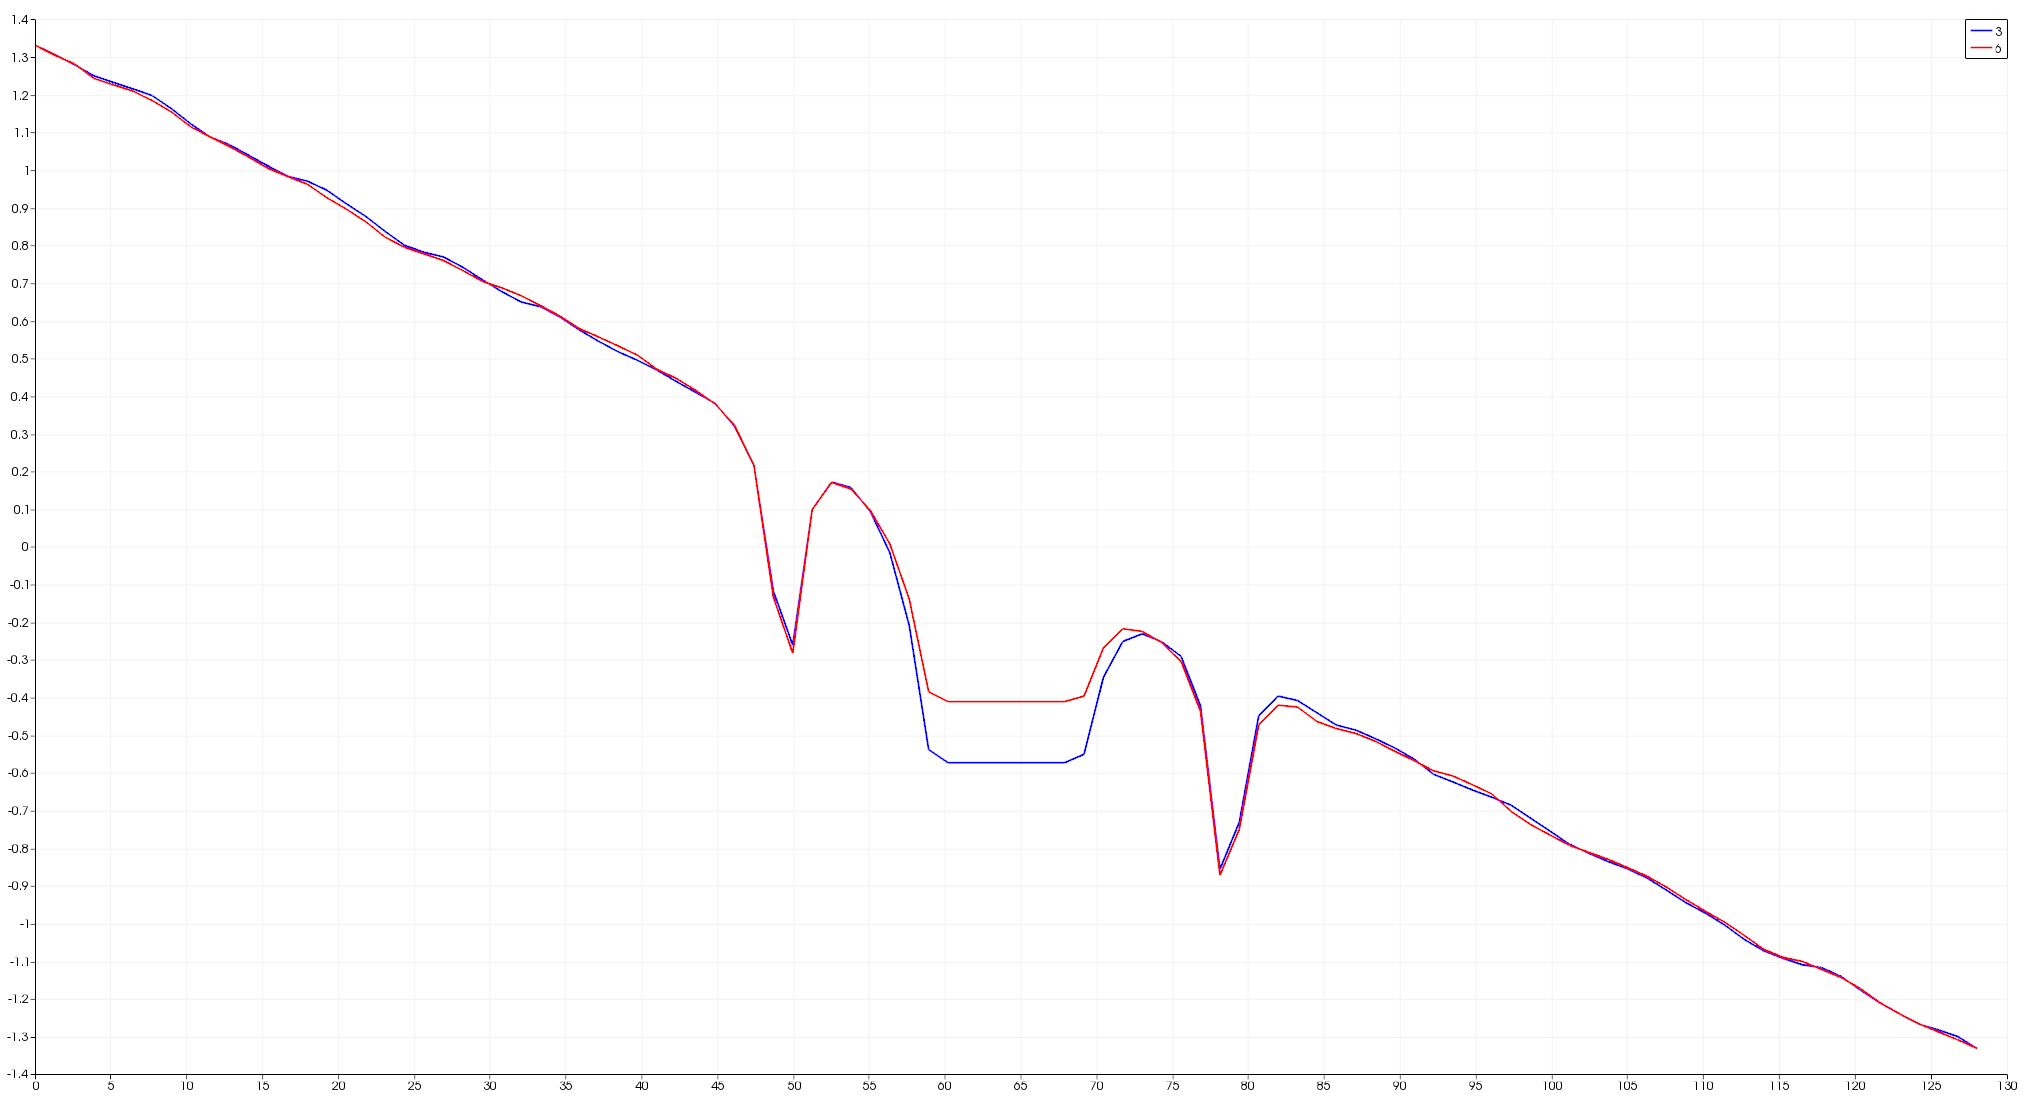
\includegraphics[width = 0.3 \textwidth]{images/pot_case36.png}
        \caption{Potential of spacecraft and surroundings with P-E and without P-E. Figure on the left displays difference between case 1 and 4. Middle figure displays difference between case 2 and 5. Rightmost figure displays difference between case 3 and 6.}
    \end{figure}
